\section{GaitNet}

\begin{todo}
  this section will show the results of training GaitNet.
  specifically, we need to show that the model is able to generate
  dynamic and acyclic gaits. We will not be comparing with the baseline
  method in this section.
\end{todo}

The primary goal of GaitNet is to generate fully dynamic and acyclic
gaits for quadruped robots. An example swing sequence can be seen in
\autoref{fig:data-swing-schedule}. This shows an acyclic
gait and dynamic gait; it is non-repetitive and the robot performs
dynamically unstable motions with up to two feet off of the ground
at once.
Additionally, the swing durations are non-uniform, with some legs
swinging for longer than others. It is clear that the system is able to
synthesize a wide variety of actions, the value of which will be evaluated
in this section.

Further analyzing \autoref{fig:data-swing-schedule}, we can see that
a particularly short step was taken by the front left leg (green) at 3s,
while a longer step was taken by the rear right leg (red) at 5s. Although
the difference in duration is minor, this shows that the system is capable
of dynamically varying the step duration.

The other takeaway from \autoref{fig:data-swing-schedule} is the
system's response to changing control inputs. Between 0-7.5s, the
system is commanded to follow a slow control input. After 7.5s, the
control input is changed to a faster speed. In the slow section,
the system is very cautious, only taking one step at a time. However,
in the fast section, the system exhibits a much more dynamic gait. At
multiple points the system can be seen to take two steps at a time,
while also not adhering to a strict alternating pattern.

\begin{todo}
  Modify figure \autoref{fig:data-swing-schedule} to show
  the terrain/robot at multiple time stamps.
\end{todo}

\begin{figure}[H]
  \centering
  \includegraphics[width=\textwidth]{images/data/swing-schedule.png}
  \caption{Example swing schedule for a single gait cycle. Each row
  represents a leg, with color indicating the leg is in swing phase.}
  \label{fig:data-swing-schedule}
\end{figure}

\autoref{fig:data-terrain-evaluation-comparison} shows the performance
of GaitNet compared to the baseline method across a variety of terrain
difficulties and commanded velocities. The results indicate that GaitNet
outperforms the baseline method in most scenarios, particularly in more
challenging terrains and at higher commanded speeds. This demonstrates
the effectiveness of GaitNet in generating robust gaits that can adapt
to varying conditions.

Further analyzing these graphs, we can see that GaitNet maintains excellent
performance when the commanded velocity is under 0.15\,m/s or the terrain
difficulty is below 5\%. ContactNet on the other hand, begins to degrade in
performance for commanded velocities above 0.05\,m/s and increasingly with
terrain difficulties. GaitNet's superior performance in these scenarios
highlights the advantages of its dynamic and acyclic gait generation
capabilities.

\begin{figure}[H]
  \centering
  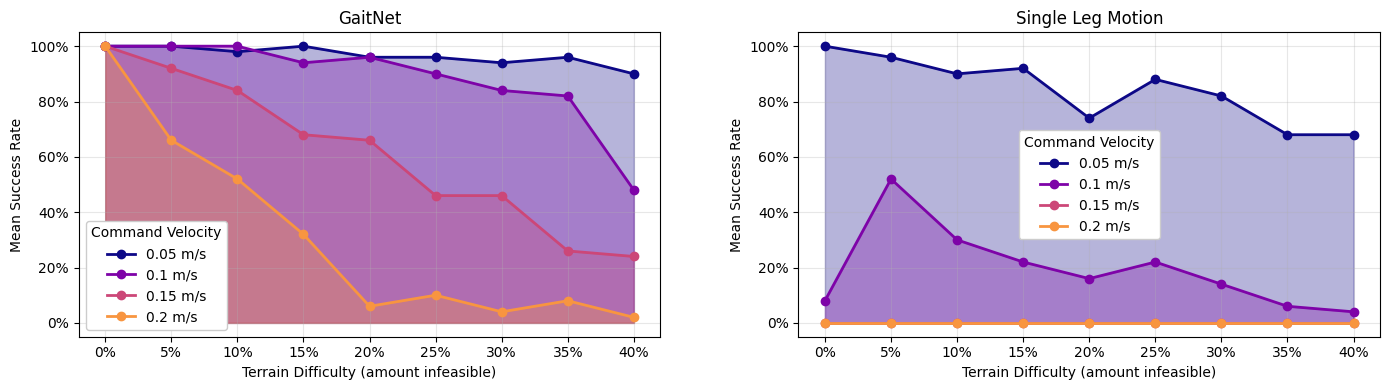
\includegraphics[width=\textwidth]{images/data/terrain-evaluation-comparison.png}
  \caption{Evaluation of GaitNet and the baseline method for
  different terrain difficulties and commanded velocities.}
  \label{fig:data-terrain-evaluation-comparison}
\end{figure}

\begin{todo}
  Include figure showing the distribution of swing durations.
\end{todo}

\begin{todo}
  Include training figures from tensorboard detailing how the model
  improves over time.
\end{todo}
